\section{Problem Formulation}

\begin{figure}[h!]
  \center
  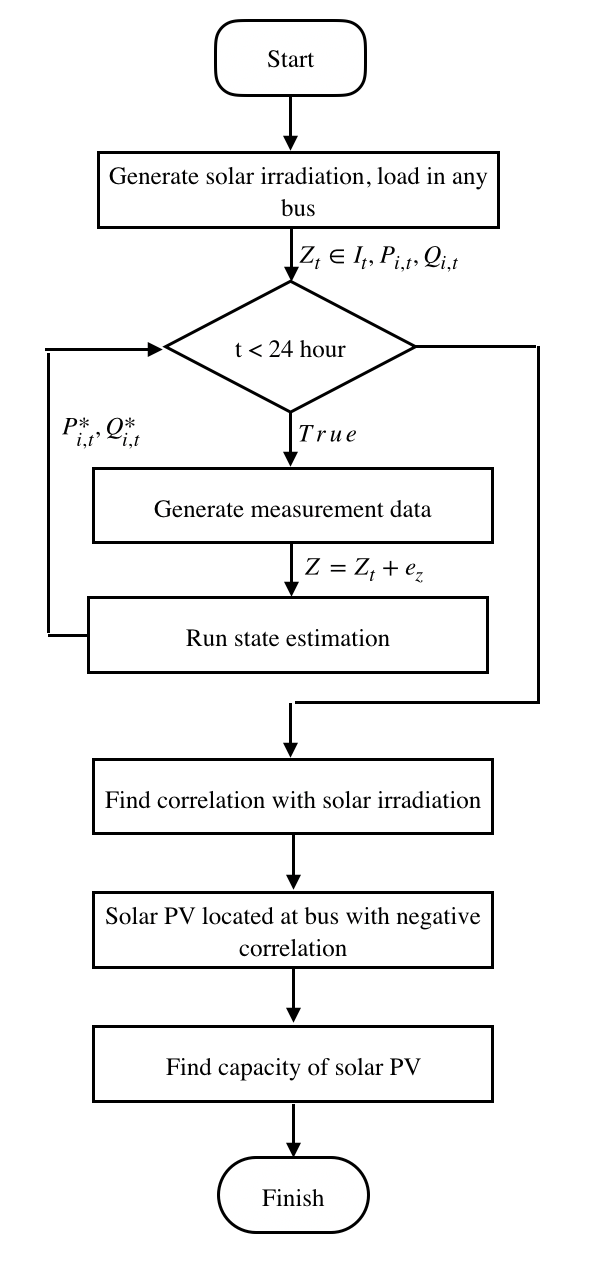
\includegraphics[scale=0.25]{images/conceptual_methodology.png}
  \caption{conceptual methodology}
  \label{fig.method}
\end{figure}

\subsection{Measurement devices, measured data and accuracy}

To generate measurement data for testing prurposes, measurement error was added to tha actual measurements as shown in Equation~\ref{eq.Z}.
\begin{equation}
  Z=Z_{a} \pm +e_{z}
\label{eq.Z}
\end{equation}
where $Z_{a}$ is actual data and $e_{z}$ is error added base on accuarcy of the measurement.
In this study, bus measurement has 3$\%$ error. line measurement has 5$\%$ error.

These error are assumed to be modeled independent Gaussian random variable\cite{b2}.
where where the error value is expected value from gaussian distribution.
noise is guassian distribution,as shown in Equation~\ref{eq.gaussian}
\begin{equation}
  g(x)=\frac{1}{\sigma \sqrt{2\pi}}e^{-\frac{1}{2}((x-\mu)/\sigma)^2}
  \label{eq.gaussian}
\end{equation}
\subsubsection{State variable description:} voltage, current, power flow from measurements devices

\subsection{Peform SE to find }
\subsubsection{LWS}
\subsubsection{Branch current, load allocation based state estimation}
is based on the weighted least square (WLS) approach\cite{b1}.
the method solves the following WLS problem to obtain an estimate ofthe system operating point defined by the system state x:
\begin{equation}
  \underset{x}{min} J(x)=\sum_{i=1}^{m}w_{i}(z_{i}-h_{i}(x))^{2}=\big[ z-h(x)\big]^{T}W\big[z-h(x)\big]
\label{eq.jacobian}
\end{equation}
where $w_{i}$ and $h_{i}(x)$ represent the weight and the measurements function associated with measurement $z_{i}$, respectively.
For the solution of this problem the conventional iterative method is adape by solving following normal equations at each iteration, to compute the update $x^{k+1}=x^{k}+\Delta x^{k}$
\begin{equation}
  \big[G(x^{k})\big]\Delta x^{k} = H^{T}(x^{k})W \big[ z-h(x^{k}) \big]
  \label(eq.delta_x)
\end{equation}

Where

\begin{equation}
  G(x)=H^{T}(x)WH(x)
  \label(eq.gain)
\end{equation}

is the gain matrix and H is the jacobian of the measurement function $h(x)$.

\subsection{Find correlation with solar irradiation}

A correlation is a statistical measure of relationship between two variables. The measure is best used in variables that demenstrate a linear relationship between each other.
The correlation coefficient that indicates the straength of the relationship between two variables can be found using following formula:

\begin{equation}
  \text{r}_{xy} =\frac{\sum(x_{i}-\overline{x})(y_{i}-\overline{y})}{\sqrt{\sum(x_{i}-\overline{y})^{2}(y_{i}-\overline{y})^{2})}}
  \label{eq.corr}
\end{equation}

where $\text{r}_{xy}$ is the correlation coefficient of the linear relationship between the variables x and y, $x_{i}$ is the values of the x-variable in a sample, $\overline{x}$ is the mean of the varialbes of the x-variable,
$y_{i}$ is the values of the y-variable in a sample, $\overline{y}$ is the mean of the varialbes of the y-variable.

The negaive correlation shows that the variables tend to move in opposity directions (i.e., when one variable increases, the other variable decreases).

\subsection{Find capacity of solar PV using changing point method}
